\documentclass{beamer}
\usepackage[utf8]{inputenc}
\usepackage[russian]{babel}
\usepackage[T2A]{fontenc}
\usepackage{amsmath}
\usepackage{amsfonts}
\usepackage{amsthm}
\usepackage{bbm}
\usepackage{amssymb}
\usepackage{bm}
\usepackage{graphicx}
\usepackage{epstopdf}
\usepackage[]{algorithm2e}
\usepackage{amsthm}

%\usetheme{Warsaw}
%\usecolortheme{sidebartab}
\usetheme{Warsaw}
\usecolortheme{seahorse}

%\definecolor{beamer@blendedblue}{RGB}{255,255,0}
%\definecolor{beamer@blendedblue}{HTML}{008A34} %green
%\definecolor{beamer@blendedblue}{HTML}{4A4A4A} %grey
%\definecolor{beamer@blendedblue}{HTML}{0E9059} %biryuz
\definecolor{beamer@blendedblue}{HTML}{027466} %blue


\theoremstyle{definition}
\newtheorem{defin}{Definition}
\newtheorem{assumption}{Assumption}
\theoremstyle{plain}
\newtheorem{thm}{Theorem}
\newtheorem{lem}{Lemma}
\newtheorem{prop}{Proposition}
\theoremstyle{remark}
\newtheorem{remark}{Remark}
\newtheorem{prob}{Problem}
\def\eqdef{\stackrel{def}{=}}

% \DeclareMathOperator*{\argmin}{argmin}
% \DeclareMathOperator*{\Argmin}{Argmin}
% \DeclareMathOperator{\barcnt}{bar}
% \DeclareMathOperator{\supp}{supp}
% \DeclareMathOperator{\est}{\mathbb{E}}
% \DeclareMathOperator{\inter}{int}
% \DeclareMathOperator{\ind}{Ind}

\begin{document}
\setlength{\abovedisplayskip}{5pt}
\setlength{\belowdisplayskip}{5pt}

	\title[\hbox to 60mm{Course project \hfill\insertframenumber\,/\,20}]
			{ Course project \\ <<Optimization approaches to community detection>>}
	\author[Igor Silin]{\large Marina Danilova, Alexander Podkopaev, Nikita Puchkin, Igor Silin}
	\institute[Affiiation]{
	\textsc{Skolkovo institute of science and technology}
	}

\date{\footnotesize{December 16, 2016}}

	\begin{frame}
		\titlepage
	\end{frame}

	\begin{frame}{Plan}
		  \tableofcontents[
		    sectionstyle=show/show,
		    subsectionstyle=show/show/show
		  ]
	\end{frame}

		% \AtBeginSection[]
		% {
		%   \begin{frame}{Plan of the following section}
		%   \tableofcontents[
		%     currentsection,
		%     sectionstyle=show/shaded,
		%     subsectionstyle=show/show/shaded
		%   ]
		%   \end{frame}
		% }
	
	\section{Introduction to community detection}

			\begin{frame}{Example}
				\vspace{-17pt}
				\center{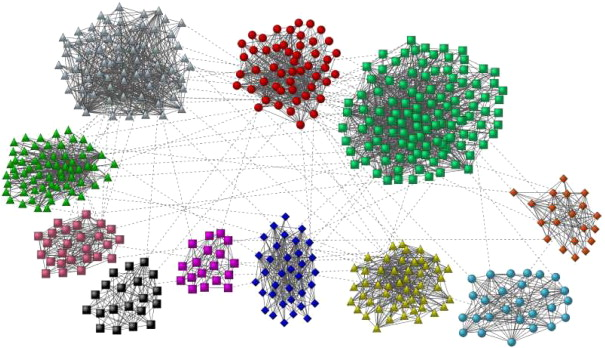
\includegraphics[width=1.0\linewidth]{images//communities.png}}
			\end{frame}
		
			\begin{frame}{Notations}

			\begin{block}{Assumption}
				We consider \textbf{undirected unweighted} graphs \textbf{without loops} with $n$ nodes.
				The nodes are enumerated as $\{ 1, ..., n\}$.\\
				Graph is given by its $n \times n $ adjacency matrix $A$.

			\end{block}

			\begin{block}{Goal of community detection}
				Find \textbf{partition} of nodes into \textbf{non-overlapping} clusters.\\
				The number of clusters is $k$.\\
				The clusters are denoted as $\{ \mathcal{C}_1, ..., \mathcal{C}_k\}$.
			\end{block}
		\end{frame}

	\section{Algorithms}
		\subsection{Spectral method}
			\begin{frame}{Spectral method}
				\begin{block}{Formulating an optimization problem}
				\end{block}
			\end{frame}

			\begin{frame}{Spectral method}
				
			\end{frame}

		\subsection{Modularity-based method}
			\begin{frame}{Modularity-based method}
				\begin{block}{Formulating an optimization problem}
				\end{block}
			\end{frame}

			\begin{frame}{Modularity-based method}
				
			\end{frame}
	
        %\subsection{Conjugate gradients method}
        \subsection{Natural conjugate gradients method}
			\begin{frame}{Natural conjugate gradients method} %{Conjugate gradients method}
                \begin{itemize}
                    \item Model parametrized by
                        \begin{equation}
                            \begin{aligned}
                            \nonumber
                                & z(i) \sim \text{Poly}(\pi), \quad i=\overline{1, n} \\
                                & P = \| p_{ij} \|_{i,j=\overline{1,k}} \text{ - probabilities of inter-cluster edges occurence} \\
                            \end{aligned}
                        \end{equation}
                
                    \item Bayesian approach:
                    \begin{equation}
                        \begin{aligned}
                        \nonumber
                            & \pi \sim \text{Dirichlet}(\alpha) \\
                            & p_{ii} \sim \text{Beta}(\beta), \quad i = \overline{1,k} \\
                            & p_{ij} \ll 1, \quad \forall i\neq j
                        \end{aligned}
                    \end{equation}
                    \item $p(z, \pi, P | A)$ - true posterior with observed adjacency matrix $A$
                    \item $\mathcal Q$ - family of feasible distributions            
                \end{itemize}

			\end{frame}

			\begin{frame}{Natural conjugate gradients method} %{Conjugate gradients method}
				\begin{block}{Formulating an optimization problem}
                    \begin{equation*}
                        \mathcal L(q) \equiv -\text{KL}\left(q \| p(Z, \pi, P | A)\right) \longrightarrow \max\limits_{q \in \mathcal Q}
                    \end{equation*}
				\end{block}
                \begin{itemize}
				    \item The problem can be reduced to unconstrained optimization:

                        \begin{equation}
                            \begin{aligned}
                            \nonumber
                            \mathcal L = \mathcal L(\theta) \longrightarrow \max, \quad \text{$\theta$ - $n\times(k-1)$ matrix}
                            \end{aligned}
                        \end{equation}

                    \item Use conjugate gradients method in a statistical manifold
                    \item Metrics is defined by a matrix
                        \[
                            \mathcal I(\theta) - \text{Fischer information}
                        \]
                \end{itemize}                
			\end{frame}

		\subsection{Semidefinite relaxations}
			\begin{frame}{Semidefinite relaxations}
				\begin{block}{Formulating an optimization problem}
				\end{block}
			\end{frame}

			\begin{frame}{Semidefinite relaxations}
				
			\end{frame}

	\section{Experimental results}
		\begin{frame}{}
				
		\end{frame}
\end{document} 